\documentclass{standalone}

\usepackage[usenames,dvipsnames]{xcolor}
\usepackage{tikz}
\usepackage{pgfplots}
\usepackage{graphicx}
\usepackage{comment}

\pgfplotsset{compat=newest}

\definecolor{IBM1}{HTML}{648fff}
\definecolor{IBM2}{HTML}{785ef0}
\definecolor{IBM3}{HTML}{dc267f}
\definecolor{IBM4}{HTML}{fe6100}
\definecolor{IBM5}{HTML}{ffb000}
\definecolor{IBM6}{RGB}{051,117,056}

\definecolor{Okabe1}{RGB}{000,158,115}
\definecolor{Okabe2}{RGB}{000,114,178}
\definecolor{Okabe3}{RGB}{086,180,233}
\definecolor{Okabe4}{RGB}{230,159,000}
\definecolor{Okabe5}{RGB}{213,094,000}
\definecolor{Okabe6}{RGB}{204,121,167}

\begin{document}
	\vspace{1cm}
		\begin{tikzpicture}
		\begin{axis}[
			%title={Diagonal View - 20 mm section},
			enlargelimits=false,
			title={$a.$},
			title style={yshift=-2ex, xshift=-31ex},
			tick pos=left, %
			tick align=outside, %
			axis line style={opacity=0}, %
			after end axis/.code={
				\draw ({rel axis cs:0,0}
				-|{axis cs:0,0}) % xmin (line starts here)
				-- ({rel axis cs:0,0}
				-|{axis cs:30,0}); % xmax (line stops here)
				\draw ({rel axis cs:0,0}
				|-{axis cs:0,0.6}) % ymin (line starts here)
				-- ({rel axis cs:0,0}
				|-{axis cs:0,1.6}); % ymax (line stops here)
			},
			legend style={at={(1,0.05)}, anchor=south east},
			xlabel={$p_i$ (kPa)},
			ylabel={$k/k_0$},
			xmin=-2.5, xmax=30,
			ymin=0.55, ymax=1.6,
			scatter/classes={
				%b={mark=*,color=Okabe6},
				c={mark=square*,mark size=3pt,color=Okabe3,fill=Okabe3!80,opacity=0.75},
				d={mark=*,mark size=3.5pt,color=Okabe5,fill=Okabe5!80,opacity=0.75}
			}
			]
			\addplot[scatter,only marks,% 
			scatter src=explicit symbolic, % Needed for scatter class styling
			error bars/.cd,
			x dir=both, x explicit,
			y dir=both, y explicit
			] 
			table[y error index=2, meta=label] {
				x y yerr label
				
				0	0.853730041	0.024127036	d
				5	0.9321147	0.038127994	d
				10	1.042876711	0.006716375	d
				15	1.055209219	0.017888792	d
				20	1.12652122	0.03217918	d
				25	1.21713215	0.032276993	d
				
				0	0.942670567	0.017280735	c
				5	1.174210231	0.038943955	c
				10	1.321660097	0.037872855	c
				15	1.367380902	0.051409677	c
				20	1.400757333	0.020391662	c
				25	1.454181999	0.037603477	c
					
			};
			%\addlegendentry[anchor=west]{Experimental}
			\addlegendentry[anchor=west,scale=0.75]{Cross Pattern}
			\addlegendentry[anchor=west,scale=0.75]{Dispersed Pattern}
			
			\node[anchor=center] at (4,1.4) {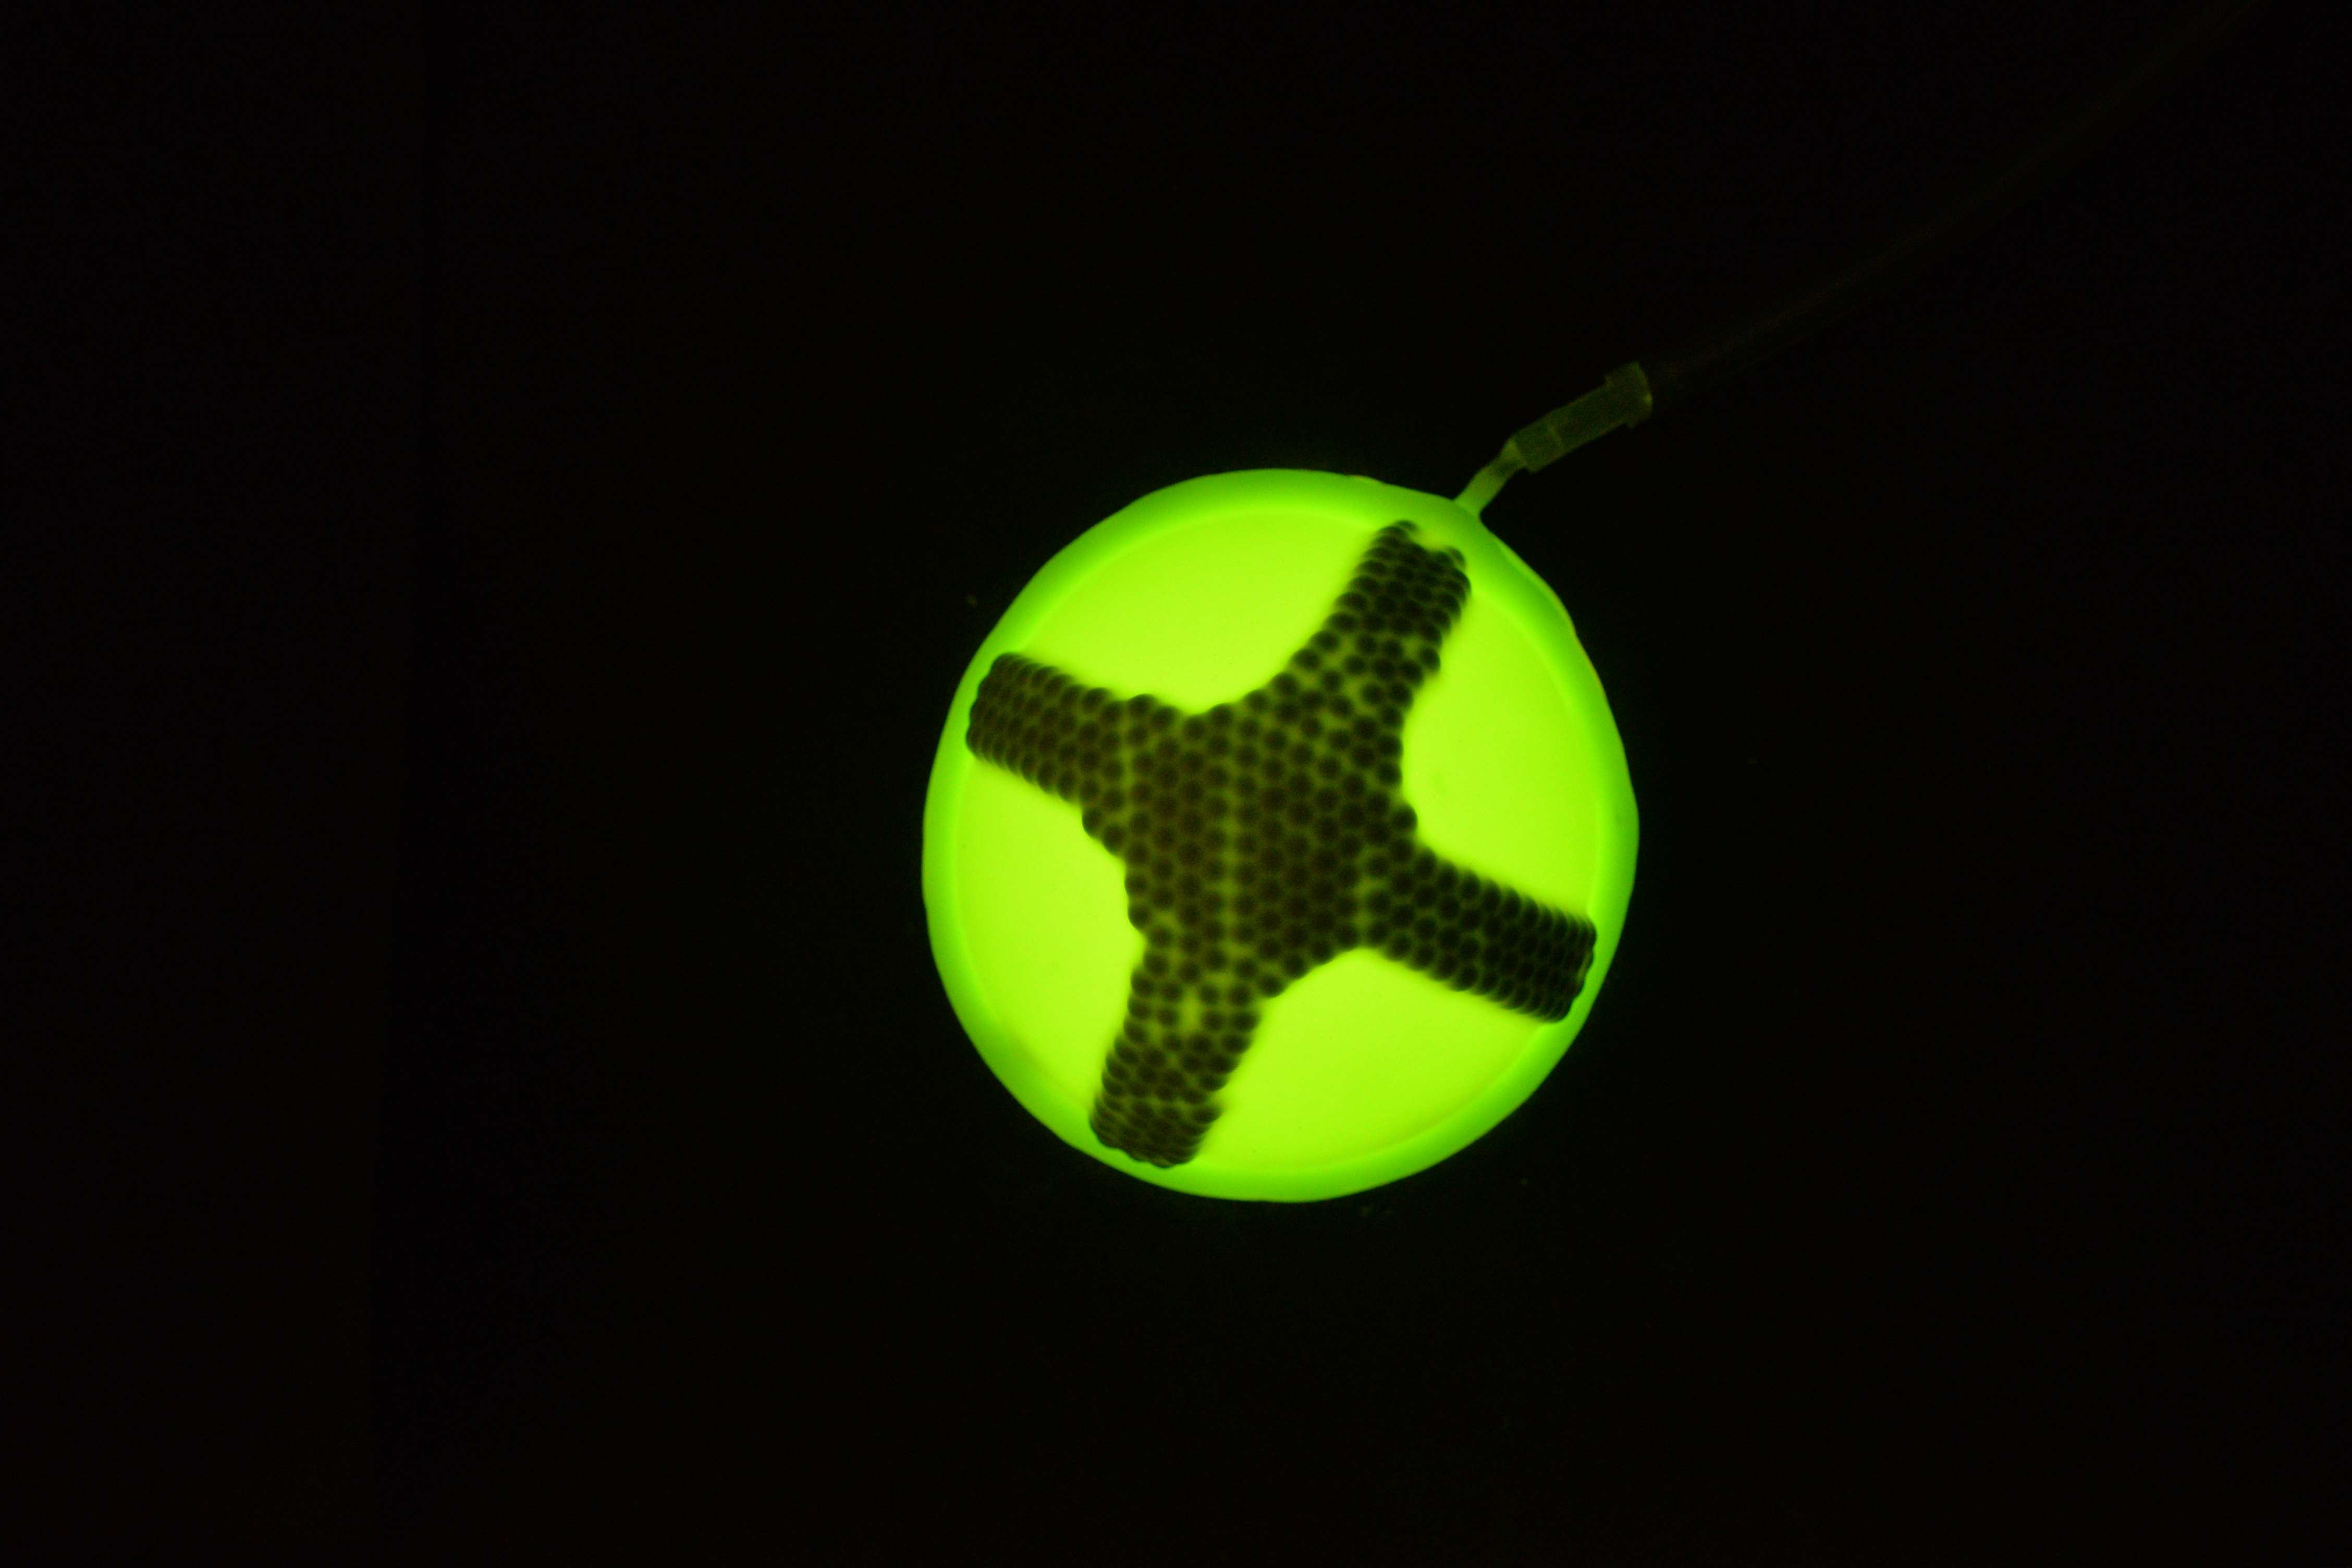
\includegraphics[width=1.5cm,trim=400 150 300 195 ,clip]{ForceChains}};
			\node[anchor=center] at (25,0.95) {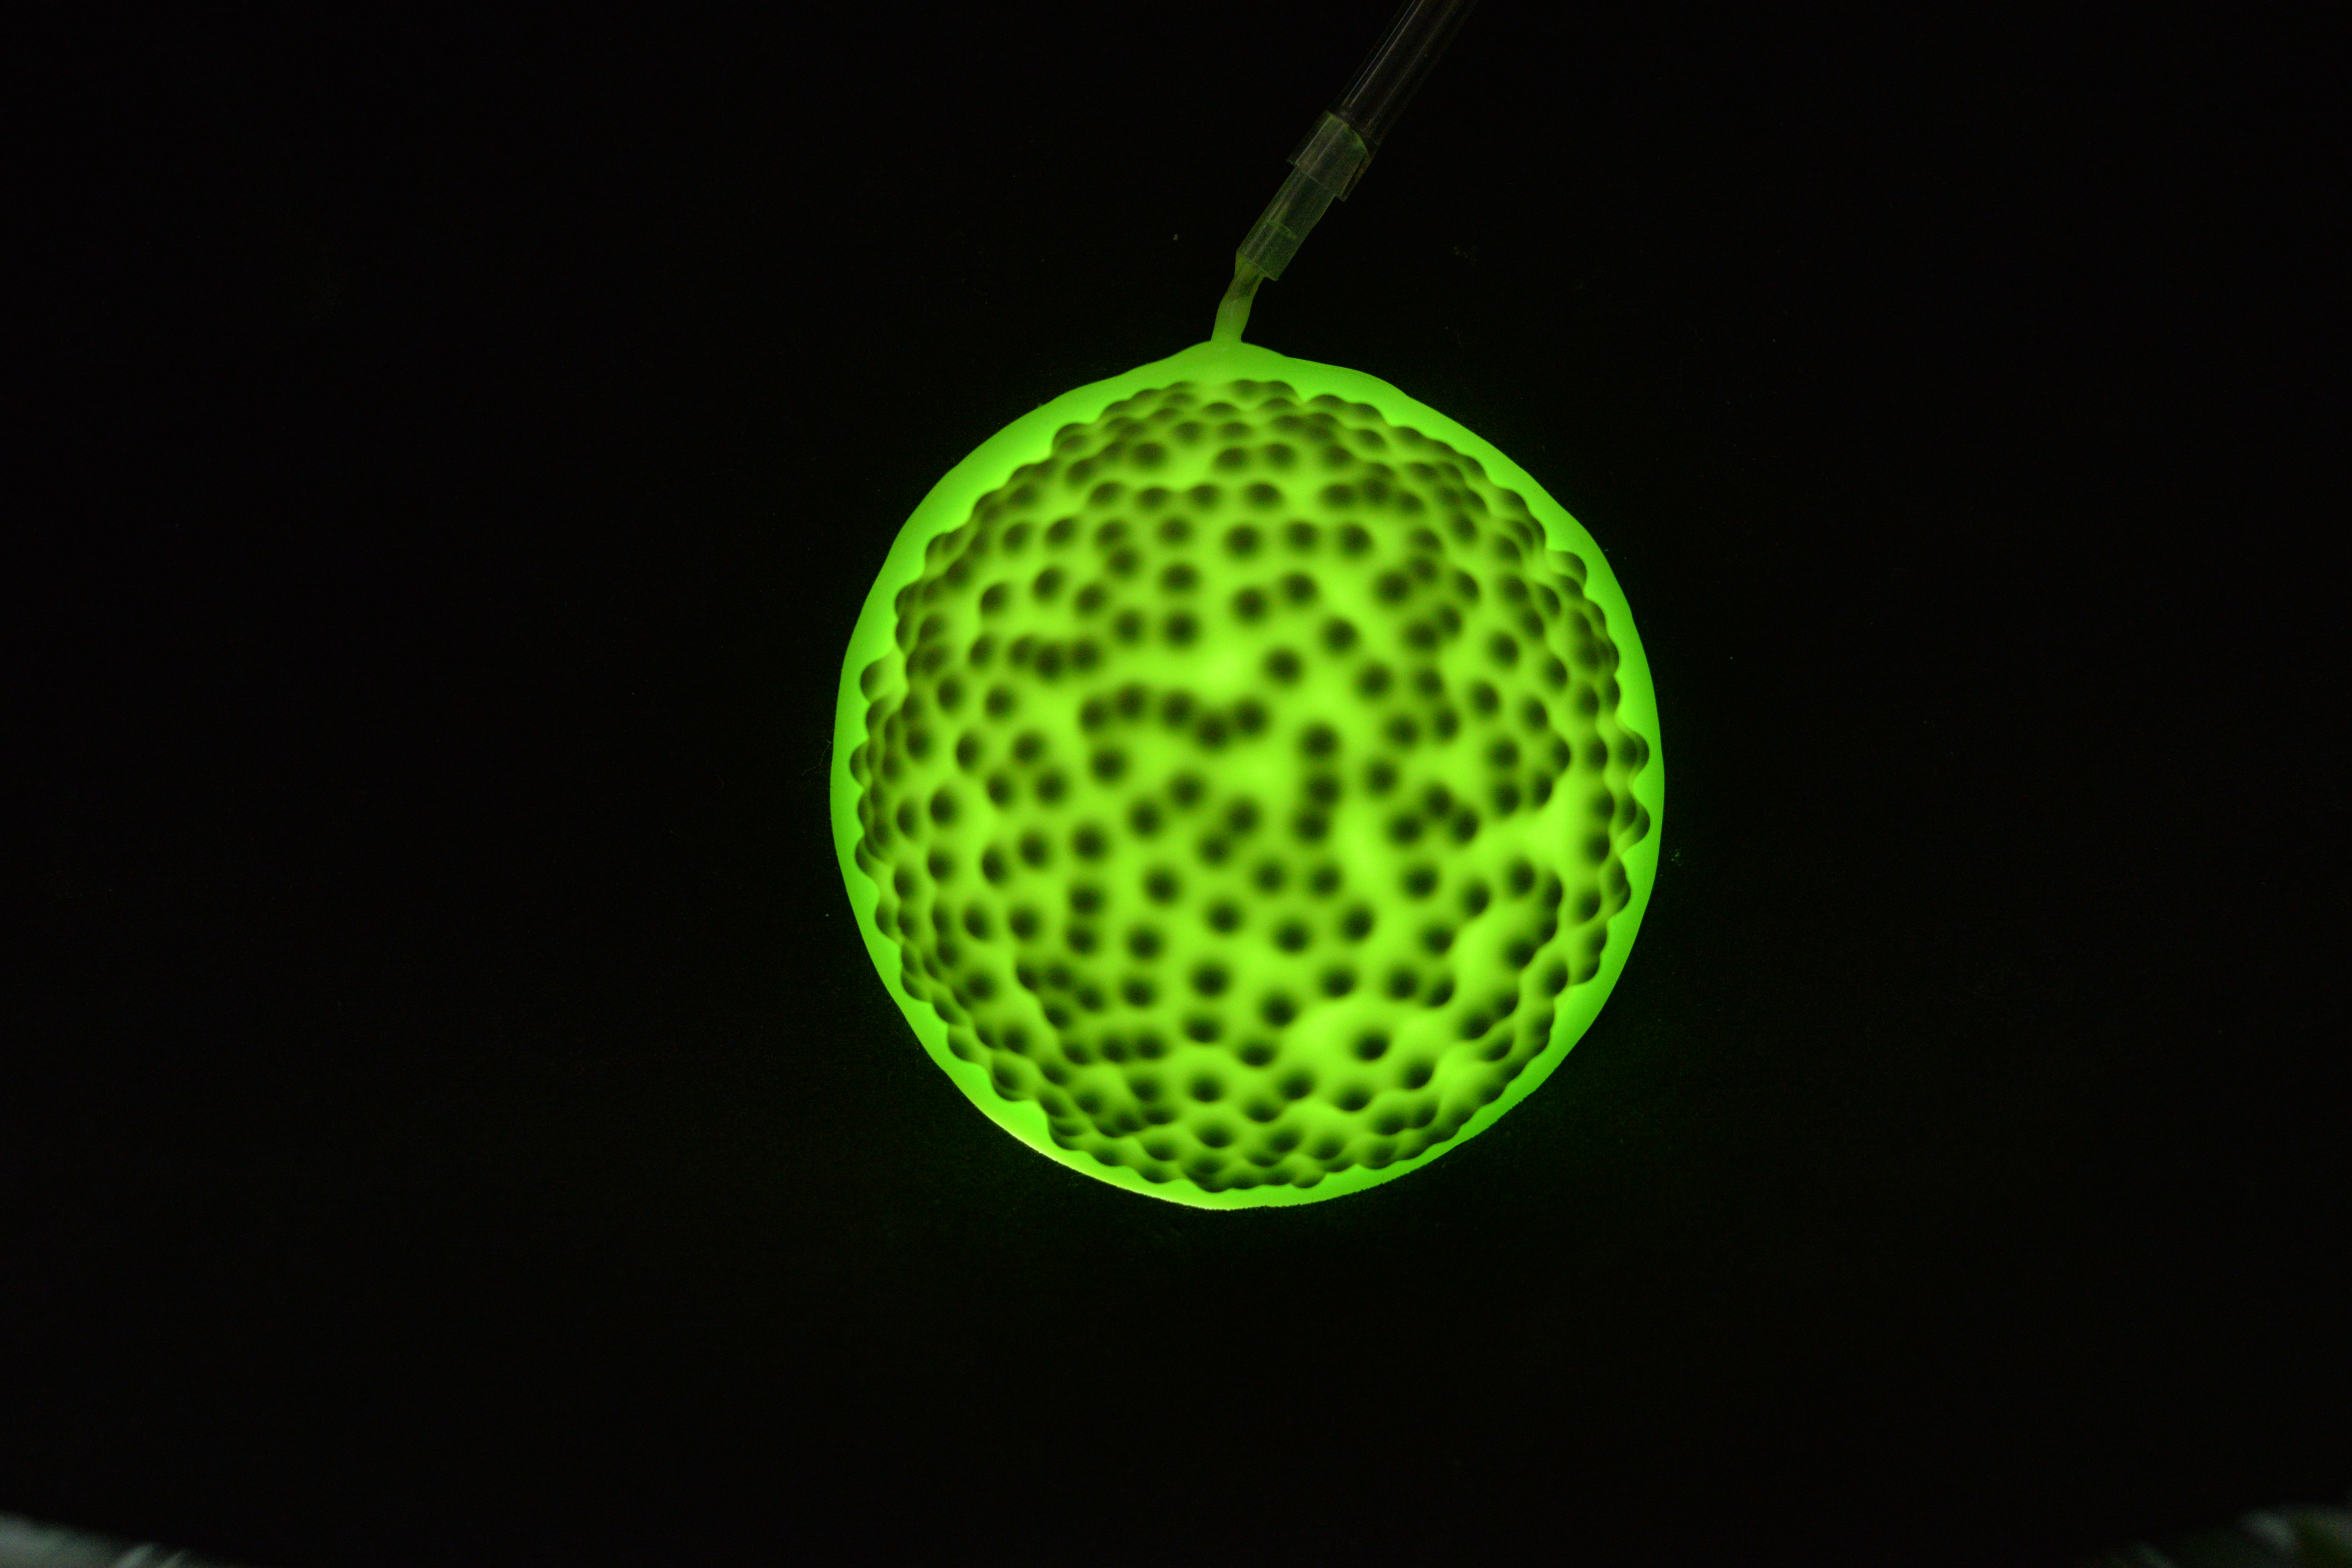
\includegraphics[width=1.5cm,trim=360 140 290 140,clip]{NoForceChains}};
			
		\end{axis}
		
	\end{tikzpicture}

	
\end{document}